\section{Exercise eight}

Consider the following code:
\begin{verbatim}
I1: LD $F1, 0($R1)
I2: FADD $F2, $F2, $F3
I3: ADDI $R3, $R3, 8
I4: LD $F4, 0(R2)
I5: FADD $F5, $F4, $F2
I6: FMULT $F6, $F1, $F4
I7: ADDI $R5, $R5, 1
I8: LD $R6, 0($R4)
I9: SD $F6, 0($R5)
I10: SD $F5, 0($R6)
\end{verbatim}
\begin{enumerate}
    \item Identify all conflicts.
    \item Develop a scoreboard for the given code, indicating clock cycles.
    \item If the previous table was incorrect, provide the accurate one, specifying the number, type, and latency for each unit.
\end{enumerate}

\subsection*{Solution}
\begin{enumerate}
    \item Conflicts:
        \begin{itemize}
        \item RAW F6 between I1 and I2
        \item RAW F2 between I2 and I3
        \item RAW F2 between I2 and I4
        \item RAW F6 between I1 and I4
        \item RAW F2 between I2 and I5
        \item WAW F0 between I3 and I5
        \item RAW F12 between I4 and I5
        \end{itemize}
    \item Scoreboard:
        \begin{figure}[H]
            \centering
            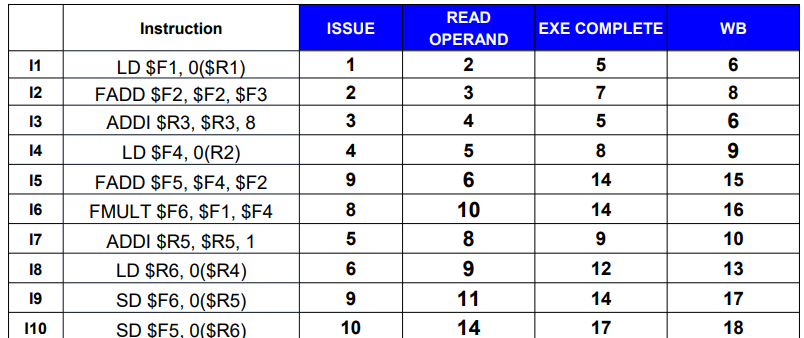
\includegraphics[width=1\linewidth]{images/score2.png}
        \end{figure}
        The issue order is incorrect, rendering the scoreboard configuration inaccurate.
    \item Correct Scoreboard:
        \begin{figure}[H]
            \centering
            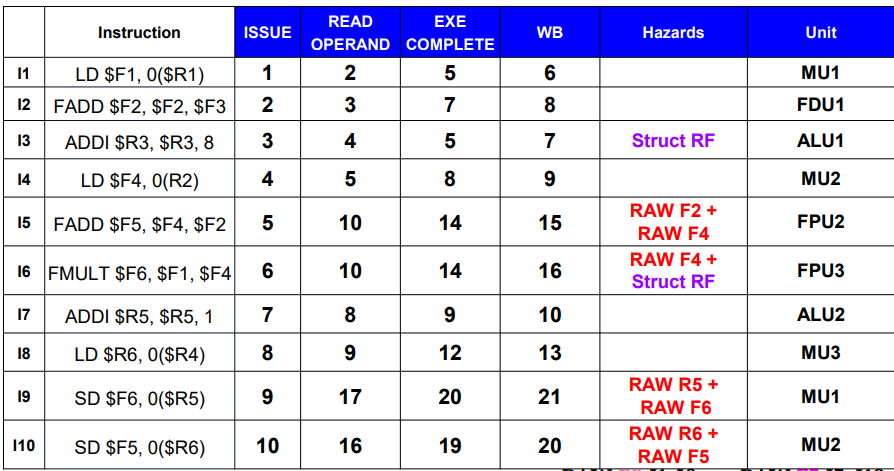
\includegraphics[width=1\linewidth]{images/score3.png}
        \end{figure}
\end{enumerate}